\documentclass[11pt]{article}
\usepackage[utf8]{inputenc}
\usepackage{dirtytalk}
\usepackage{mathrsfs}
\usepackage{blindtext}
\usepackage{csquotes}
\usepackage{mathtools} 	
\usepackage{polynom}
\usepackage{amsthm}
%for the rendering of maths
\numberwithin{equation}{section}					
%reset numbering within a structural object
\numberwithin{figure}{section}						
%reset numbering within a structural object
 \usepackage{natbib}
\usepackage[margin=1.5cm]{geometry}
\usepackage{url}
\usepackage{amssymb,amsmath,graphics}
\title{\textbf{Taller Introducción a la Teoría de Conjuntos \\El Cardinal del Continuo}}
\author{Edgar Santiago Ochoa Quiroga\\
\date{}
}

\begin{document}
\maketitle
\renewcommand\qedsymbol{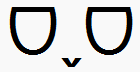
\includegraphics[height=2ex]{Demo face.png}}
\begin{enumerate}
   \item Demuestre que el conjunto de todos los conjuntos finitos de reales tiene cardinal de $2^{\aleph_0}$.
   \begin{proof}[\textbf{Solución}]
   Denotemos $\textbf{F}$ el conjunto de todos los conjuntos finitos de reales y definamos el siguiente conjunto:
   \begin{equation*}
       F_1=\{\{x\}:x\in\mathbb{R}\}
   \end{equation*}
   Es fácil darse cuenta que $F_1\subset\textbf{F}$. Luego ya teniendo esto en cuenta note que podemos definir la función $f:F_1\longrightarrow\textbf{F}$ tal que $f(\{x\})=\{x\}$, en pocas palabras la identidad, note que $f$ es inyectiva por lo tanto $|F_1|\leq|\textbf{F}|$.\\
   Ahora considere la siguiente función $g:\mathbb{R}\longrightarrow F_1$ tal que $g(x)=\{x\}$, esta función claramente es biyectiva y se puede concluir que $|F_1|=|\mathbb{R}|=2^{\aleph_0}$, de esta forma tenemos que:
   \begin{equation*}
       2^{\aleph_0}\leq|\textbf{F}|
   \end{equation*}
   De forma inmediata consideramos el conjunto $F_2=\{\{x_0,x_1\}:x_i\in\mathbb{R}\}$, es decir el conjunto de subconjuntos de $\mathbb{R}$ con $2$ elementos, note que podemos definir una inyección $h:F_2\longrightarrow\mathbb{R}^2$ tal que $h(\{x_0,x_1\})=(x_0,x_1)$ por lo tanto $|F_2|\leq|\mathbb{R}^2|=|\mathbb{R}|^2=(2^{\aleph_0})^2=2^{\aleph_0}$, note que podemos generalizar este argumento para un conjunto $F_k=\{\{x_0,x_1,\dotsc,x_{k-1}\}:x_i\in\mathbb{R}\}$ de la misma manera podemos definir una función inyectiva $h_k:F_k\longrightarrow\mathbb{R}^k$ por lo tanto todo conjunto de subconjuntos finitos de reales tiene por mucho el cardinal de los reales es decir $|F_k|\leq2^{\aleph_0}$ y ahora demostremos que:
   \begin{equation*}
      \textbf{F}=\bigcup\limits_{k=0}^nF_k
   \end{equation*}
   Primero notemos que todo elemento de $F_k$ es un subconjunto finito de reales, luego se tiene que cada $F_k\subseteq\textbf{F}$ y por tanto $\bigcup\limits_{k=0}^nF_k\subseteq\textbf{F}$. Tomemos $A\in\textbf{F}$ eso quiere decir que $A$ es un conjunto finito de reales por la definición de $\textbf{F}$, luego $A\in F_k$ para algún $F_k$ y por tanto $A\in\bigcup\limits_{k=0}^nF_k$. Como hemos probado que son iguales entonces se debe de tener que $|\textbf{F}|=|\bigcup\limits_{k=0}^nF_k|$ pero notemos que 
   \begin{equation*}
       |\bigcup\limits_{k=0}^nF_k|=\sum\limits_{k=0}^n|F_k|=|F_0|+|F_1|+\dotsc+|F_n|\leq2^{\aleph_0}+2^{\aleph_0}+\dotsc+2^{\aleph_0}\leq\aleph_0\cdot2^{\aleph_0}=2^{\aleph_0}
   \end{equation*}
   De esta forma concluimos que $|\textbf{F}|\leq2^{\aleph_0}$ y por el teorema de Cantor-Bernstein tenemos que $|\textbf{F}|=2^{\aleph_0}$.
   \end{proof}
   \item Muestre que el conjunto de todos los números algebraicos es contable y por tanto el conjunto de todos los números trascendentales tiene cardinal de $2^{\aleph_0}$.
   \begin{proof}[\textbf{Solución}]
   Consideremos el conjunto:
   \begin{equation*}
    \mathcal{P}_n=\{p(x):p(x)=a_nx^n+a_{n-1}x^{n-1}+\dotsc+a_1x+a_0\text{ con }a_i\in\mathbb{Z}\}   
   \end{equation*}
   Note que para un polinomio de grado $n$ el conjunto $\{a_0,a_1,\dotsc,a_{n-1},a_n\}$ tiene $n+1$ elementos, entonces tenemos que $(a_0,a_1,\dotsc,a_{n-1},a_n)\in\mathbb{Z}^{n+1}$ por lo tanto definamos una función $f:\mathbb{Z}^{n+1}\longrightarrow\mathcal{P}_n$ tal que $f(a_0,a_1,\dotsc,a_{n-1},a_n)=a_nx^n+a_{n-1}x^{n-1}+\dotsc+a_1x+a_0$, note que por mera definición de los polinomios de grado $n$ siempre va a existir una $n+1$-tupla con sus coeficientes correspondientes y por tanto es sobreyectiva. Ahora para mostrar que es inyectiva suponga que $f(a_0,a_1,\dotsc,a_{n-1},a_n)=f(b_0,b_1,\dotsc,b_{n-1},b_n)$ luego $a_nx^n+a_{n-1}x^{n-1}+\dotsc+a_1x+a_0=b_nx^n+b_{n-1}x^{n-1}+\dotsc+b_1x+b_0$ y recordemos que dos polinomios son iguales si los coeficientes de cada potencia son iguales y por tanto se tiene que $(a_0,a_1,\dotsc,a_{n-1},a_n)=(b_0,b_1,\dotsc,b_{n-1},b_n)$, de esta forma concluimos que $f$ es biyectiva y por tanto $|\mathcal{P}_n|=|\mathbb{Z}^{n+1}|$ luego como $\mathbb{Z}^{n+1}$ es un producto finito de conjuntos contables ya que $|\mathbb{Z}|=|\mathbb{N}|$ tenemos que $|\mathbb{Z}^{n+1}|=|\mathbb{N}|$ y como es relación de equivalencia tenemos que $|\mathcal{P}_n|=|\mathbb{N}|$ y por tanto $\mathcal{P}_n$ es contable.\\
   Ahora consideremos para cada $p(x)\in\mathcal{P}_n$ el conjunto $A_n(p(x))=\{x\in\mathbb{R}:p(x)=0\}$ note que por definición que todo elemento de $A_n(p(x))$ es un numero algebraico y a su vez recordemos que todo polinomio tiene a lo mas $n$ soluciones por lo tanto $A_n(p(x))$ es finito. y consideremos:
   \begin{equation*}
       A_n=\bigcup\limits_{p(x)\in\mathcal{P}_n}A_n(p(x))
   \end{equation*}
   Note que esta es una unión contable de conjuntos finitos por lo tanto $A_n$ es contable. Denotemos $\mathbb{A}$ como el conjunto de números algebraicos y demostremos que:
   \begin{equation*}
       \mathbb{A}=\bigcup\limits_{n=1}^{\infty}A_n
   \end{equation*}
   Primero note que que todo elemento de cada $A_n$ es un numero algebraico por lo tanto es bastante evidente que cada $A_n\subseteq\mathbb{A}$ y por lo tanto $\bigcup\limits_{n=1}^{\infty}A_n\subseteq\mathbb{A}$.
   Tomemos $x_1\in\mathbb{A}$ por definición de número algebraico existe un polinomio de algún grado tal que $p(x)\in\mathcal{P}_n$ y $p(x_1)=0$ luego por definición del conjunto $x_1\in A_n(p(x))$ y por tanto $x_1\in A_n$. Luego como $\mathbb{A}$ es la unión contable de conjuntos contables quiere decir que es contable, es decir $|\mathbb{A}|=|\mathbb{N}|$.\\
   Por ultimo recordemos que $\mathbb{A}\subseteq\mathbb{R}$ y además $|\mathbb{R}|=2^{\aleph_0}$ luego por un teorema mencionado en el libro se tiene que $|\mathbb{R}-\mathbb{A}|=2^{\aleph_0}$ y note que el conjunto definido por $\mathbb{R}-\mathbb{A}$ es el conjunto de los números trascendentales y de esta forma concluimos la demostración.
   \end{proof}
   \item Si un conjunto ordenado linealmente $P$ tiene un subconjunto denso contable, entonces $|P|\leq2^{\aleph_0}$.
   \begin{proof}[\textbf{Solución}]
   Sea $(P,<)$ y $D\subseteq P$ denso en $P$ y contable, consideremos la función $f:P\longrightarrow\mathcal{P}(D)$ tal que $f(p)=\{d\in D:d<p\}$, primero notemos que para todo $p\in P$ se tiene que $f(p)\subseteq D$ y por lo tanto $f(p)\in\mathcal{P}(D)$ por lo que esta bien definida. 
   Ahora demostremos que $f$ es inyectiva, supongamos $x,y\in P$ y $x\neq y$, como $P$ esta linealmente ordenado $x<y$ ó $y<x$, sin perdida de generalidad trabajemos con el caso $x<y$, como $D$ es denso en $P$ tenemos que existe un $z\in D$ tal que $x<z<y$, luego como $z\in D$ y $z<y$ tenemos que $z\in f(y)$ pero como $x<z$ se tiene que $z\notin f(x)$ y por axioma de extensionalidad $f(x)\neq f(y)$.\\
   De esta forma hemos demostrado que $|P|\leq|\mathcal{P}(D)|$ pero por aritmética cardinal tenemos que $|\mathcal{P}(D)|=2^{|D|}=2^{\aleph_0}$ ya que $D$ es contable y por tanto $|P|\leq2^{\aleph_0}$.
   \end{proof}
   \item El conjunto de todos los subconjuntos cerrados de reales tiene cardinal de $2^{\aleph_0}$.
   \begin{proof}[\textbf{Solución}]
   Sea $\mathcal{C}$ el conjunto de todos los subconjuntos cerrados de $\mathbb{R}$ y $\mathcal{A}$ el de los abiertos, definamos la función $F:\mathcal{C}\longrightarrow\mathcal{A}$ tal que $F(D)=\mathbb{R}-D$, primero note que para todo $D\in\mathcal{C}$ se tiene que $\mathbb{R}-D=F(D)\in\mathbb{A}$ por lo que esta bien definida.\\
   Consideremos $X,Y\in\mathcal{C}$ y $X\neq Y$, sin perdida de generalidad supongamos que existe al menos un elemento $a$ tal que $a\in X$ y $a\notin Y$ luego note que evidentemente $a\in\mathbb{R}$ ya que $X$ es un subconjunto cerrado de reales, por definición de diferencia entre conjuntos tenemos que $a\notin\mathbb{R}-X$ y $a\in\mathbb{R}-Y$ y por extensionalidad tenemos que $F(X)=\mathbb{R}-X\neq\mathbb{R}-Y=F(Y)$ mostrando que $F$ es inyectiva.\\
   Ahora sea $Y\in\mathcal{A}$ y consideremos $X=\mathbb{R}-Y$ note que $X\in\mathcal{C}$ por lo que podemos aplicar $F$ teniendo que $F(X)=\mathbb{R}-(\mathbb{R}-Y)=\mathbb{R}\cap Y=Y$, como $Y$ es arbitrario podemos asegurar que todo $Y\in\mathcal{A}$ se tiene que $Y=F(X)$ y por tanto $F$ es sobreyectiva. De esta forma hemos demostrado que $F$ es biyectiva y por lo tanto $|\mathcal{C}|=|\mathcal{A}|$ pero por un teorema del libro tenemos que $|\mathcal{A}|=2^{\aleph_0}$ luego como la equipotencia es una relación de equivalencia concluimos que $|\mathcal{C}|=2^{\aleph_0}$.
   \end{proof}
   \item Muestre que para $n>0$, $n\cdot2^{2^{\aleph_0}}=\aleph_0\cdot2^{2^{\aleph_0}}=2^{\aleph_0}\cdot2^{2^{\aleph_0}}=2^{2^{\aleph_0}}\cdot2^{2^{\aleph_0}}=(2^{2^{\aleph_0}})^n=(2^{2^{\aleph_0}})^{\aleph_0}=(2^{2^{\aleph_0}})^{2^{\aleph_0}}=2^{2^{\aleph_0}}$.
   \begin{proof}[\textbf{Solución}]
    Note que por las propiedades de la aritmética cardinal y las propiedades de los alephs podemos plantear las siguientes secuencias de desigualdades:
    \begin{equation*}
    2^{2^{\aleph_0}}\leq n\cdot2^{2^{\aleph_0}}\leq\aleph_0\cdot2^{2^{\aleph_0}}\leq2^{\aleph_0}\cdot2^{2^{\aleph_0}}\leq2^{2^{\aleph_0}}\cdot2^{2^{\aleph_0}}=2^{2^{\aleph_0}+2^{\aleph_0}}=2^{2^{\aleph_0}}   
    \end{equation*}
    \begin{equation*}
    2^{2^{\aleph_0}}\leq(2^{2^{\aleph_0}})^n\leq(2^{2^{\aleph_0}})^{\aleph_0}\leq(2^{2^{\aleph_0}})^{2^{\aleph_0}}=2^{2^{\aleph_0}\cdot2^{\aleph_0}}=2^{2^{\aleph_0}}   
    \end{equation*}
    Luego por el teorema de Cantor-Bernstein y el hecho de que la cardinalidad es una relación de equivalencia se obtiene el resultado.
   \end{proof}
   \item El cardinal del conjunto de todas las funciones discontinuas es $2^{2^{\aleph_0}}$.
    \begin{proof}[\textbf{Solución}]
   Primero notemos que $|\mathbb{R}^\mathbb{R}|=|\mathcal{C}|+|\mathcal{D}|$ siendo $\mathcal{C}$ el conjunto de funciones continuas de $\mathbb{R}$ en $\mathbb{R}$ y $\mathcal{D}$ el conjunto de funciones discontinuas de $\mathbb{R}$ en $\mathbb{R}$, ahora recordemos que $|\mathbb{R}^\mathbb{R}|=2^{2^{\aleph_0}}$ y que $|\mathcal{C}|=2^{\aleph_0}$, note que $|\mathcal{D}|\leq|\mathbb{R}^\mathbb{R}|$ debido a que podemos definir $F:\mathcal{D}\longrightarrow\mathbb{R}^\mathbb{R}$ tal que $f\longmapsto f$ es decir la identidad y evidentemente esta función es inyectiva.\\
   Ahora supongamos que $|\mathcal{D}|<|\mathbb{R}^\mathbb{R}|$ luego tenemos que $|\mathcal{C}|+|\mathcal{D}|<|\mathcal{C}|+|\mathbb{R}^\mathbb{R}|$ y por la aritmética cardinal y el ejercicio anterior tenemos que:
   \begin{equation*}
       2^{2^{\aleph_0}}<2^{\aleph_0}+2^{2^{\aleph_0}}<2^{2^{\aleph_0}}+2^{2^{\aleph_0}}=2\cdot2^{2^{\aleph_0}}=2^{2^{\aleph_0}}
   \end{equation*}
   Implicando que $2^{2^{\aleph_0}}<2^{2^{\aleph_0}}$, una contradicción. De esta forma podemos concluir que $|\mathcal{D}|=|\mathbb{R}^\mathbb{R}|$, es decir $|\mathcal{D}|=2^{2^{\aleph_0}}$.
   \end{proof}
   \begin{proof}[\textbf{Solución usando A.E.}]
   Primero recordemos de nuevo el hecho de que $|\mathbb{R}^\mathbb{R}|=|\mathcal{C}|+|\mathcal{D}|$ y como $|\mathcal{C}|=2^{\aleph_0}$ esto implica que $\mathcal{C}$ es infinito y por lo tanto podemos aplicar el resultado usando axioma de elección tal que $|\mathcal{C}|+|\mathcal{D}|=\text{max}\{|\mathcal{C}|,|\mathcal{D}|\}=|\mathbb{R}^\mathbb{R}|$ y como conocemos el tamaño de $\mathcal{C}$ y de $\mathbb{R}^\mathbb{R}$ tenemos que $\text{max}\{2^{\aleph_0},|\mathcal{D}|\}=2^{2^{\aleph_0}}$ y como $2^{\aleph_0}<2^{2^{\aleph_0}}$ se debe de tener que $|\mathcal{D}|=2^{2^{\aleph_0}}$. 
   \end{proof}
   \item Construya una función biyectiva de $\mathbb{R}\times\mathbb{R}$ en $\mathbb{R}$.
   \begin{proof}[\textbf{Solución}]
   Utilizando la idea proporcionada por el libro con unas cuantas alteraciones ya que es bien conocido que $|\mathbb{R}|=|(0,1)|$ entonces definiremos la función $f:(0,1)\times(0,1)\longrightarrow(0,1)$ de la siguiente manera:\\
   Primero consideremos la pareja de elementos $(a,b)$ tal que $a,b\in(0,1)$ note que cada elemento de ese intervalo puede ser escrito por su expresión decimal, por ejemplo podemos considerar $\frac{1}{7}=0.1428571\dots$ y $\frac{1}{9}=0.111111\dots$ luego tomamos la pareja $(0.1428571\dots,0.111111\dots)$ y al evaluar obtenemos:
   \begin{equation*}
       f(0.1428571\dots,0.111111\dots)=0.11412181517111\dots
   \end{equation*}
   Ahora la pregunta es que exactamente fue lo que definimos como función, básicamente considerando dos números de la forma $a=0.a_0a_1a_2a_3\dots$ y $b=0.b_0b_1b_2b_3\dots$, definimos $f(a,b)$ tal que:
   \begin{equation*}
       f(0.a_0a_1a_2a_3\dots,0.b_0b_1b_2b_3\dots)=0.a_0b_0a_1b_1a_2b_2a_3b_3\dots
   \end{equation*}
   Pero para hacerlo de esta forma tenemos que definir unas cuantas restricciones.\\
   Primero notemos que $\frac{1}{2}=0.5\overline{0}$ y además $\frac{1}{2}=0.4\overline{9}$ esto primero causaría que para un numero tuviera dos imágenes distintas por lo que en todos los casos tomaremos la representación con $9$ periódica y ahora el intercalar los términos los haremos por bloques de términos precedidos por ceros, para esto consideremos el siguiente ejemplo:
   \begin{equation*}
       f(0.00340700006\dots,0.08999\dots)=0.\mathbf{003}08\mathbf{4}9\mathbf{07}9\mathbf{00006}9\dots
   \end{equation*}
   Note que lo que hacemos es si hay una tira finita de ceros extendemos el bloque hasta que aparezca el dígito distinto al $0$  y si no hay tiras de ceros si hacemos el intercalado usual. Es fácil ver que esta función es sobreyectiva ya que como cada elemento del intervalo $(0,1)$ tiene una expresión decimal que lo representa es decir para todo $z\in(0,1)$ se tiene que:
   \begin{equation*}
       z=0.00z_00z_10000z_2z_30z_40z_5\dots
   \end{equation*}
   con tiras finitas de ceros arbitrarias y números arbitrarios repartidos pero nunca una tira de ceros infinitas por tanto separando los bloques obtenemos que:
   \begin{align*}
       0.00z_00z_10000z_2z_30z_40z_5\dots\Rightarrow0.\mathbf{00z_0 }0z_1\mathbf{0000z_2 }z_3\mathbf{z_4 }0z_5\dots\\
       f(0.00z_0000z_2z_4\dots,0.0z_1z_30z_5\dots)=0.\mathbf{00z_0 }0z_1\mathbf{0000z_2 }z_3\mathbf{z_4 }0z_5\dots
   \end{align*}
  Aunque no sea tan claro la inyectividad también se tiene ya que si consideramos las parejas $(a,b)=(c,d)$ note que $a=c$ y $b=d$ por tanto ambas tienen la misma escritura en decimales y por tanto al intercalar los bloques las dos expresiones serán iguales y por tanto $f(a,b)=f(c,d)$, concluyendo finalmente que $f$ si es biyección.
   \end{proof}
\end{enumerate}

\end{document}
